\documentclass[tikz]{standalone}

\usetikzlibrary{external}
%\tikzexternalize

\begin{document}

\begin{tikzpicture}[x = 1pt, y = 1pt]
\draw (-100, -100) rectangle (100, 100);
\draw[fill = red] (0, 0) circle (30);
\end{tikzpicture}
\newpage

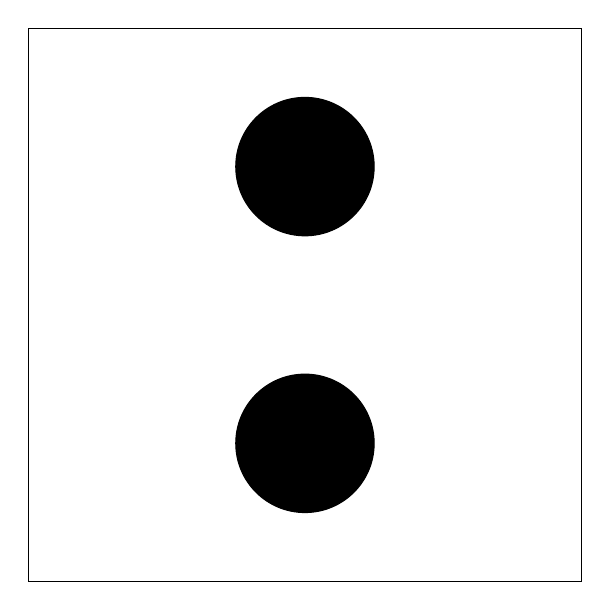
\begin{tikzpicture}[x = 1pt, y = 1pt]
\draw (-100, -100) rectangle (100, 100);
\draw[fill = black] (0, 50) circle (25);
\draw[fill = black] (0, -50) circle (25);
\end{tikzpicture}
\newpage

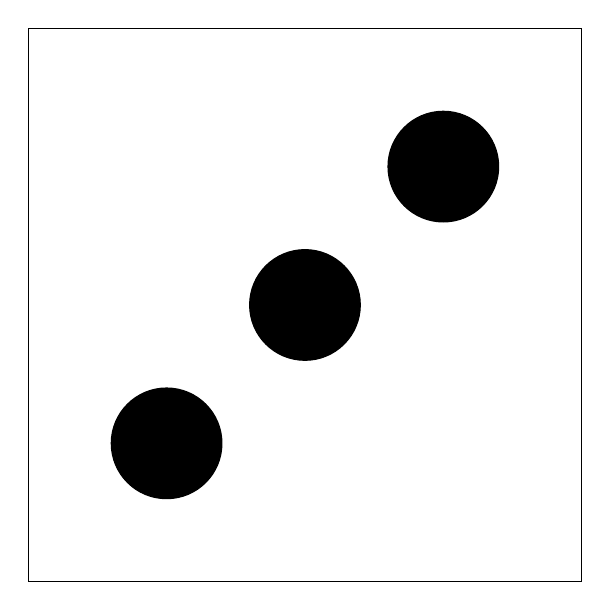
\begin{tikzpicture}[x = 1pt, y = 1pt]
\draw (-100, -100) rectangle (100, 100);
\draw[fill = black] (-50, -50) circle (20);
\draw[fill = black] (0, 0) circle (20);
\draw[fill = black] (50, 50) circle (20);
\end{tikzpicture}
\newpage

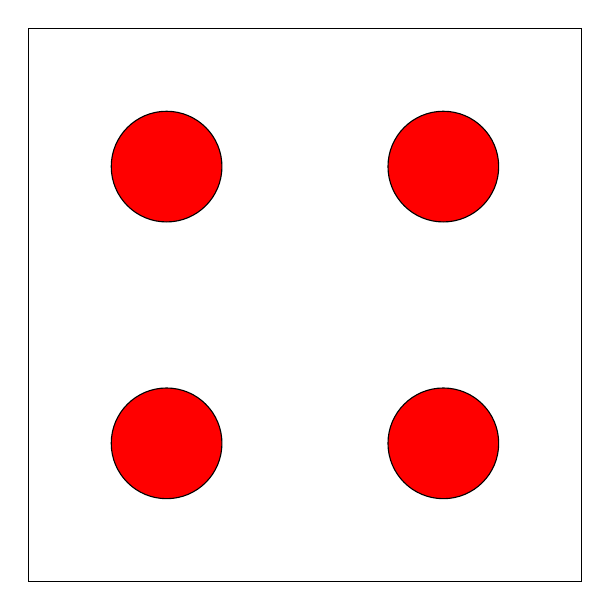
\begin{tikzpicture}[x = 1pt, y = 1pt]
\draw (-100, -100) rectangle (100, 100);
\draw[fill = red] (-50, -50) circle (20);
\draw[fill = red] (50, -50) circle (20);
\draw[fill = red] (-50, 50) circle (20);
\draw[fill = red] (50, 50) circle (20);
\end{tikzpicture}
\newpage

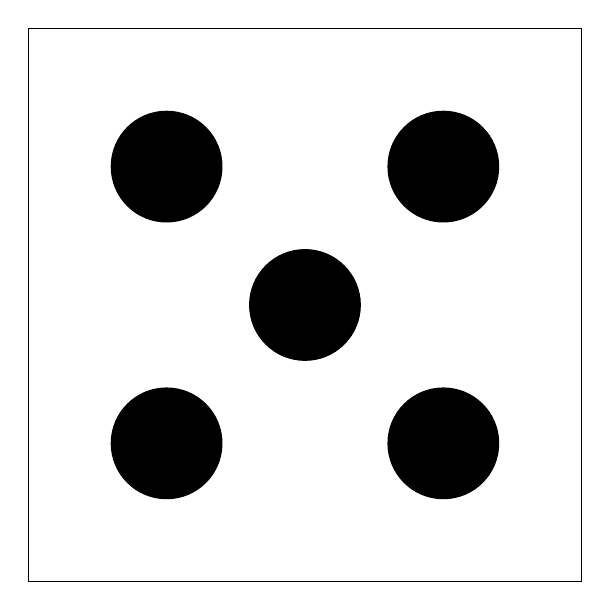
\begin{tikzpicture}[x = 1pt, y = 1pt]
\draw (-100, -100) rectangle (100, 100);
\draw[fill = black] (-50, -50) circle (20);
\draw[fill = black] (50, -50) circle (20);
\draw[fill = black] (-50, 50) circle (20);
\draw[fill = black] (50, 50) circle (20);
\draw[fill = black] (0, 0) circle (20);
\end{tikzpicture}
\newpage

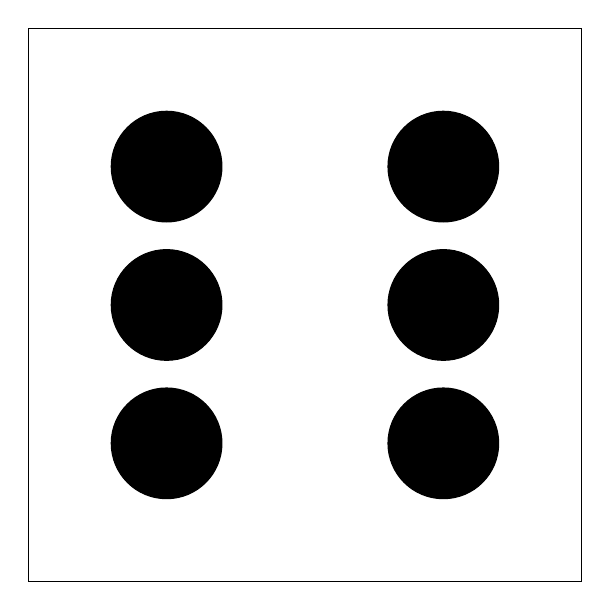
\begin{tikzpicture}[x = 1pt, y = 1pt]
\draw (-100, -100) rectangle (100, 100);
\draw[fill = black] (-50, -50) circle (20);
\draw[fill = black] (-50, 0) circle (20);
\draw[fill = black] (-50, 50) circle (20);
\draw[fill = black] (50, -50) circle (20);
\draw[fill = black] (50, 0) circle (20);
\draw[fill = black] (50, 50) circle (20);
\end{tikzpicture}
\newpage
\end{document}
